\chapter{Software}

\label{ch:chapter4}


The results stated here were originally published in paper \cite{Extasy2016} and paper \cite{Extasy2019} including the figures in this chapter.


paper extasy1, software part of extasy2
asynch

The accurate sampling of protein dynamics is an ongoing challenge despite
the utilization of \GRE{High-Performance} Computers (HPC) systems. Utilizing only "brute
force" MD simulations requires an unacceptably long time to solution. Adaptive
sampling methods allow a more effective sampling of protein dynamics than
standard MD simulations. Depending on the restarting strategy the speed up can
be more than one order of magnitude. One challenge limiting the utilization of
adaptive sampling by domain experts is the relatively high complexity \GRE{of
efficiently running adaptive sampling} on HPC systems. We discuss how the ExTASY framework can
set up new adaptive sampling strategies, and reliably execute resulting
workflows at scale on HPC platforms. Here the folding dynamics of three small
proteins \GRE{are} predicted with no a priori information.
\end{abstract}
\section{\label{sec:intro}Introduction}

Molecular dynamics (MD) simulations with all-atom force-fields allow simulating
protein folding and protein kinetics with good accuracy. Reaching biologically
relevant processes, such as protein folding or drug binding, is limited mainly
by the required large computational resources and long simulation times. The
long simulation times can be reduced either by simulating parallel trajectories
with massively-distributed computing \cite{DistComp-Shirts2000,
DistComp-Buch2010} or with special-purpose hardware \cite{shaw2014anton}.
Further reduction of required computational resources or simulation times would
allow a more broad application of MD simulations.

One method of reducing both the computational resources and the simulation times is \emph{adaptive sampling} \cite{singhal2005error, bowman2010enhanced,
weber2011characterization, Fabritiis-2014, preto2014fast, doerr2016htmd,
AdaptivePELE-Lecina2017, EvolutionCoupling-Shamsi2017, FAST-Bowman-2015, 
Strategies-erros-reduce, plattner2017complete, Adstrategies2018}. 
Adaptive sampling is an iterative process, where MD simulations from previous
iterations are analyzed, and, based on the analysis, a new iteration of relatively
short MD trajectories is initiated. The starting conformations for the
MD trajectories are determined in such a way to efficiently
reach a goal such as crossing rare transitions barriers, folding a protein, or
recovering the dynamics of a macromolecule. The exact strategy where to restart
new MD simulations determines the success of the adaptive sampling approach,
and several different methods have been proposed and investigated\GRE{\cite{Fabritiis-2014,
AdaptivePELE-Lecina2017, preto2014fast, doerr2016htmd,
weexplore, prattWESTPAAdvancesSampling2018, Adstrategies2018, FUNN, FAST}. One approach is to select new restarting configurations based on the PCA projection of the already sampled configurations \cite{shkurti2019jctc,harada2015jctc,harada2017jctc}.} Adaptive sampling
requires to use multiple parallel simulations and is therefore suitable for
High-Performance Computers (HPC).

Determining the efficiency, accuracy, and reliability of a particular adaptive
sampling strategy is challenging for several reasons. Different proteins can
behave differently for different adaptive sampling strategies but limited
computational resources don't allow to adaptively sample a statistically
significant number of proteins with different strategies for comparison.
Accurate results are known only for a limited number of proteins. Despite
these challenges some performance analyzes of adaptive sampling strategies
have been performed
\cite{preto2014fast,weber2011characterization,bowman2010enhanced,Fabritiis-2014,
Adstrategies2018}. The results show that some adaptive sampling strategies are
both reliable, accurate and reach speed ups of one or more orders of magnitude
\GRE{compared to} plain MD. For a larger, more complex protein a higher speed up is expected \cite{Adstrategies2018}.

An important challenge in adaptive sampling simulations is the complexity of
performing the required computational tasks efficiently on HPC platforms with
heterogeneous software and hardware environments. This complexity can detract
from the core objective of investigating the behavior of a particular protein
or the efficiency of new adaptive sampling strategies. Some of the existing
frameworks which currently strive to reduce this entry-barrier to
adaptive sampling, such as HTMD\cite{doerr2016htmd} and SSAGES \cite{SSAGES},
are either bound to specific software packages, algorithms, computing
platforms or are not open source. \GRE{DeepDriveMD \cite{leeDeepDriveMDDeepLearningDriven2019} allows to utilize deep learning in adaptive sampling similar to ExTASY, but DeepDriveMD hasn't released it's code yet.  The additional sampling frameworks involving neural networks \cite{jung2019acp, ribeiro2018tjocp, bonati2019pnasu} show the effective sampling of toy systems and small peptides.} In contrast, the ExTASY\cite{Extasy2016}
framework \GRE{is shown to work for proteins larger than small peptides, scales to 1000s of GPUs and is not limited to specific software packages. ExTASY supports multiple adaptive sampling
algorithms, different dimension reduction methods} and is extensible to new algorithms and methods while being open source and agnostic of the HPC platform. In addition to a demonstration of the
scientific results that can be achieved by using ExTASY, in this manuscript, we
investigate the advantages of scalability, reliability or reproducibility
arising from ExTASY framework for adaptive sampling.

% and the framework used in this manuscript, ExTASY. Despite the availability
% of these frameworks, in many cases the adaptive sampling in current research
% is not performed on any of them, in most cases not reaching the maximum

\section{\label{sec:methods}Methods}

Many different implementations of adaptive sampling exist but they all 
have in common
that the previous MD simulations are analyzed and restart points for the next
batch of MD simulations are determined from the analysis of the sampled configurational space.
The different implementations mainly differ in the analysis step, and
they can be based on Markov State Models (MSMs) \cite{prinz2011markov,
MSM-Pande-2018,bookmsm,masterequationsMSM,SCHUTTE1999146}, Diffusion Maps
\cite{Coifman7426, rohrdanz2011determination,Zheng2011, Boninsegna2015},
likelihood-based approaches \cite{peters2006obtaining}, cut-based free energy
profiles \cite{krivov2008diffusive}, or neural networks
\cite{Mardt2018,wehmeyer2018time, ribeiro2018reweighted}. 
In this manuscript, we exemplify the
usage of the ExTASY framework with Markov State Models with different restarting
strategies, as described in Section~\ref{sec:restart-strategies}.

\subsection{\label{sec:adaptive-sampling} Adaptive Sampling}

In each iteration of Markov State Models-based adaptive sampling, all previous
MD simulations are analyzed.
Figure~\ref{fig:schema} is a graphical representation of the process. In the
first iteration of the adaptive sampling, the MD simulations are generated from
the system starting state as shown in Step 1.

In Step 2 all previous trajectories are analyzed. \GRE{The first step is dimension reduction. One dimension reduction approach is using} Time-lagged
Independent Component Analysis (TICA) \cite{TICA1-perez2013, TICA2-schwantes2013} converts the raw trajectories in
low-dimensional trajectories. The Koopman method \cite{koopmanold,
koopman2,koopman3,koopman4, wu2017variational, Nueske2017} is used to reduce
the non-equilibrium effects emerging from collecting many short MD trajectories. The
resulting low-dimensional trajectories are scaled into a kinetic map
\cite{Noe2015,noe2016commute}, which provides a measure of the kinetic distance
between different configurations. \GRE{Another dimension reduction approach implemented by default in ExTASY is a deep learning approach with state-free reversible VAMPnets (SRV) \cite{Mardt2018,chen2019jcp}. The SRVs can effectively achieve non-linear dimension reductions. The SRV originates from the same variational
approach to conformational dynamics as TICA. The trajectory and the time-lagged trajectories are transformed with a neural network into dimension reduced trajectories. The dimension reduced trajectories are then used to calculate the VAMP-2 score, which is used as the loss function for the backpropagation to optimize the parameters of the neural network. The non-linear dimension reduction achieved with SRV improves the separation of different states. On advantage of SRVs is that SRVs can reach the same accuracy for time scales with shorter lag times than TICA. For adaptive sampling, the shorter lag time for analysis allows increasing the frequency of restarting trajectories which potentially improves adaptive sampling. In this case, the length of MD trajectories in each iteration is reduced and the number of iterations is increased.} 

\GRE{The dimension reduced trajectories are then} clustered with k-means into approximately 200 microstates,
the detailed values for each protein are provided in the Supplementary Information. 
A  maximum-likelihood estimation with a detailed balance
constraint \cite{prinz2011markov} allows obtaining an MSM transition matrix 
between every pair of microstates. All the analysis was
performed using the PyEMMA Python package \cite{scherer2015pyemma}, which
allows fast adjustments in the analysis step. The exact parameters for the MSM
construction for each protein are listed in the
Supplementary Information. All these steps can be modified or replaced easily in the
ExTASY workflow. 

\begin{figure}[h]
  \centering
  \includegraphics[width=0.9\linewidth]{figures2/schema1.pdf}
  \caption{The flow chart shows the basic structure of adaptive sampling. The
  number of starting conformations is variable. The software and hardware
  generating the MD simulations are variable. Different Analysis methods in Step 2
  are possible, commonly TICA \cite{TICA1-perez2013, TICA2-schwantes2013} and
  MSM \cite{prinz2011markov} are used, but alternative methods such as Vampnet \cite{Mardt2018}
  are possible. In Step 3 the goal can be also variable, from finding the whole protein
  dynamics to exploring smaller-scale changes. Step 4 allows different adaptive
  sampling strategies such as the FAST method \cite{FAST} or the strategies
  discussed in this work.}
  \label{fig:schema}
\end{figure}

\begin{figure}[h]
  \centering
  \includegraphics[width=0.9\linewidth]{figures2/asynch.pdf}
  \caption{\GRE{Asynchronous, concurrent execution of the individual molecular dynamics and analysis tasks. The Step 4 in Figure~\ref{fig:schema} uses the restarting conformations from the latest available analysis results.}}
  \label{fig:asynch}
\end{figure}

The overall adaptive sampling process described in Figure~\ref{fig:schema} can be summarized as follows:
\begin{itemize}
\item Start: Start with a start conformation. In the cases presented here, we
start from \GRE{one unfolded configuration specified in Section~\ref{sec:MD}}.
\item Step 1: Generate a batch of molecular dynamics trajectories from the
selected conformations, the parallelization is defined by the available
computational resources. This step is described in Section~\ref{sec:MD}.
\item Step 2: analyze the all available data as described in
Section~\ref{sec:adaptive-sampling}, using the probabilities from the MSM
transition matrix.
\item Step 3: Decide if the goal of adaptive sampling is achieved. In this
work, the goal is finding the folded state and obtaining a converged equilibrium
dynamics for the protein. If the goal is not achieved, proceed to Step 4;
otherwise, stop the iterative process.  
\item Step 4: Select the batch of protein conformations for Step 1 in the next
iteration as described in Section~\ref{sec:restart-strategies}.
\end{itemize}

After Step 2 the adaptive sampling continues with Step 4 if the goal is not
achieved. This goal could be folding the protein, achieving a pre-determined
accuracy of the protein dynamics, but could also be manually set to finish
after several iterations. If the goal is not achieved in Step 3, in Step 4 
a batch of protein conformations for the next iteration is selected as
described in Section~\ref{sec:restart-strategies}. If the goal in Step 3 is
achieved, the iterative adaptive sampling finishes and the trajectories can be
further analyzed. 

\GRE{ExTASY allows to execute the iterative process in Figure~\ref{fig:schema} in both synchronous and asynchronous manner. In the synchronous case, the previous step has to be finished to proceed with the next step. The disadvantage of synchronous execution is the lower utilization of computational resources since most of the GPUs won't perform any calculations while the Steps 2-4 are executed. The asynchronous case as shown in Figure~\ref{fig:asynch} is designed to increase the utilization of computational resources by continually updating the restarting configurations for the next MD step by continually rerunning the analysis step. When one MD trajectory finishes, the MD worker will retrieve the last generated restarting configuration for the next MD trajectory and immediately start the next MD trajectory. This significantly reduces the downtime for the MD workers. The disadvantage of the asynchronous approach is that the analysis processes only a fraction of the MD trajectories from the last iteration since these MD trajectories aren't finished when the analysis starts. These trajectories will be fully analyzed only in the next iteration. To reduce the unanalyzed length of the trajectories the analysis step has to be continuously rerun, shown in Figure~\ref{fig:asynch}.  In this paper, all the results are executed asynchronously. The ability of asynchronous execution is a significant advantage over other adaptive sampling packages.}

\subsection{\label{sec:restart-strategies}Restart Strategies for Adaptive Sampling}


\begin{figure}[h!]
  \includegraphics[width=0.48\textwidth]{figures2/extasy_arch_coarse.pdf}
  \caption{ExTASY-EnTK Integration: The diagram illustrates
  the seven execution steps of an adaptive sampling algorithm using ExTASY.  
  }\label{fig:extasy_arch}
\end{figure}

In the ExTASY framework, the different Restart Strategies in Step 4 in
Figure~\ref{fig:schema} are easily exchangeable. Here we use \GRE{two
strategies, the first one is the Macrostate Count based strategy, further called $cmacro$
strategy, and the second one is the} Microstate Count based strategy, further called $cmicro$
strategy. \GRE{The $cmacro$ strategy was shown to be more effective in reaching the
folded state of the protein and the} $cmicro$ strategy was shown to be \GRE{particularly}
effective in exploring the whole protein landscape \cite{Adstrategies2018}. 
\GRE{These strategies do} not assume any a priori knowledge of the system except
the chemical structure of the unfolded protein, but other adaptive sampling
strategies that use additional information about the protein can be used in
the ExTASY framework.

\paragraph{Adaptive sampling strategy $cmicro$}
One simple restart strategy is starting new molecular dynamics trajectories in
the microstates which have the worse statistics, that is, that have been visited the least during prior iterations
\cite{weber2011characterization, Fabritiis-2014, AdaptivePELE-Lecina2017,
doerr2016htmd}. This statement can be quantified by using the counts in the count matrix of the MSM from Step 2,
that report on how many times all previous trajectories have visited each
microstate.  The probability that any given microstate is selected in Step 4 for
the batch of restart conformations is inversely proportional to its associated count. The $cmicro$ strategy is effective in quickly exploring new regions of the whole protein landscape and to better sample the protein dynamics \cite{Adstrategies2018}.


\paragraph{\label{sec:macro} Adaptive sampling strategy $cmacro$} 
Another popular restart strategy for adaptive sampling is a macrostate-based
method indicated here as $cmacro$. The main advantage of this
method is the faster folding of proteins or crossing of transition barriers
\cite{Adstrategies2018}. This advantage is achieved by using eigenvectors of
the on-the-fly MSM from Step 2 to select more restart configurations in areas which are
kinetically disconnected or less explored. In this method, the microstates of
the on-the-fly MSM are clustered into macrostates, for
example with PCCA \cite{roblitz2013fuzzy}. Any microstate not connected in the
main MSM is treated as an additional macrostate. The number of macrostates can
be either fixed, as in this work or determined based on the number of
slow processes emerging from the analysis. The macrostate count is determined by
measuring how many times any previous trajectory has visited each macrostate.
The restart conformations for the next iteration of adaptive sampling are then
chosen from each macrostate inversely proportional to the macrostate count.
Individual conformations within a macrostate are selected inversely
proportional to the microstate count within the macrostate.

\subsection{\label{sec:Tools}Tools and Software}
\begin{figure}[h!]
    \begin{lstlisting}
    from @radical.entk@ import @Task, Stage, Pipeline@
    p = Pipeline()

    sim_stage = Stage()   
    sim_task = Task()
    sim_task.executable = @<executable>@ #example openmm
    sim_task.arguments = <args> #example openmm args
    <add other task properties>
    sim_stage.add_tasks(sim_task)
    
    ana_stage = Stage()
    ana_task = Task()
    ana_task.executable = @<executable>@ #example pyemma
    ana_task.arguments = <args> #example pyemma args
    <add other task properties>
    
    ana_stage.add_tasks(ana_task)
    ana_stage.post_exec = {
        'condition': eval_sims(),
        'on_true':   add_sims(),
        'on_false':  terminate()
        }
    
    p.add_stages([sim_stage, ana_stage])
    \end{lstlisting}
    \caption{Pseudocode describing the adaptive sampling algorithm using the
    EnTK API}\label{extasy_snippet}
\end{figure}


ExTASY is a domain-specific workflow
system~\cite{turilli2019middleware,turilli2018building} for adaptive sampling
algorithms on HPC platforms. ExTASY exposes domain-specific parameters and
simulation configurations, but abstracts complexities of execution management,
resource acquisition, and management using RADICAL-Cybertools
(RCT)~\cite{Balasubramanian2019rct}. RCTs are software systems designed and
implemented in accordance with the building blocks approach
\cite{turilli2018building}. Each system is independently designed with
well-defined entities, functionalities, states, events, and errors.
Specifically, ExTASY uses Ensemble Toolkit
(EnTK)~\cite{balasubramanian2018harnessing} and RADICAL-Pilot
(RP)~\cite{merzky2018using}. Ensemble
Toolkit~\cite{entk-icpp-2016,balasubramanian2018harnessing} provides the
ability to create and execute ensemble-based applications with complex
coordination and communication but without the need for explicit resource
management.  EnTK uses RP~\cite{merzky2018using}, which provides resource
management and task execution capabilities. In this section, we describe the
ExTASY framework and how it leverages capabilities offered by EnTK and RP.



\subsubsection{ExTASY}



ExTASY exposes configuration files to interface with users and two components:
Composer and Descriptor.

The Composer validates the user input and creates the Resource, Execution
Pattern, Simulation, and Analysis sub-components. The Resource represents a
valid resource description; Execution Pattern describes the number of
iterations, number of simulation tasks per iteration and number of analysis
tasks per iteration; Simulation and Analysis describe the parameters to be
used for simulation and analysis tasks.

The Descriptor interfaces with Ensemble Toolkit, the execution middleware. It
consists of two sub-components: Resource Descriptor and Application
Descriptor. The former converts the resource description to a format as
accepted by the middleware. The latter uses the information from the Execution
Pattern, Simulation and Analysis sub-components to describe the complete
application to be executed.


Figure~\ref{fig:extasy_arch} presents the integration between ExTASY and the
execution middleware (EnTK). ExTASY translates the adaptive sampling
application into ordered executable tasks through a series of events: ExTASY
parses the configurational files to determine parameters to be used and
creates Resource description (event 1) and the simulation and analysis tasks
to be executed (event 2). ExTASY then uses EnTK's interface to describe the
resource and application (event 3 and 4) and initiate execution on the target
resource (event 5 and 6). EnTK executes all the simulations and analysis on
the resource (event 7).


ExTASY uses EnTK programming abstractions and EnTK's application programming
interface (API). ExTASY also uses EnTK's capabilities to support adaptive
execution~\cite{balasubramanian2019adaptive} by modifying the execution plan
depending upon intermediate results e.g., add more simulations and analysis
tasks. Figure~\ref{extasy_snippet} provides pseudo-code on how ExTASY
implements an adaptive sampling algorithm using the EnTK API.


\subsubsection{Ensemble Toolkit \& RADICAL-Pilot}

EnTK simplifies the creation and execution of applications with complex
ensemble coordination and communication requirements. EnTK decouples the
description of ensemble coordination and communication from their execution by
separating three distinct concerns: (i) specification of task and resource
requirements; (ii) resource acquisition and management; and (iii) task
execution.



EnTK enables the encoding of ensemble applications by exposing an API with
four components: Application Manager, Pipeline, Stage and Task. Users specify
their application using pipelines, stages, and tasks. Users then pass this
specification and description of the target resource to the Application
Manager. Resource description includes properties like wall-time, number of
nodes and credentials for resource access.

The Task component is used to encapsulate an executable and its software
environment. The Stage component contains a set of tasks without mutual 
dependencies and that can therefore be executed concurrently. The Pipeline 
component is used to describe a sequence of stages. Description of ensemble
applications in terms of concurrency and sequentiality avoids the need to 
explicitly specify dependencies between tasks.

EnTK supports an explicit definition of pre and post conditions on the
execution of tasks, enabling fine-grained
adaptivity~\cite{balasubramanian2019adaptive}. Adaptivity allows modifications
to the number, type and order of tasks to be executed during runtime, based on
intermediate results. Specifically, EnTK supports three types of adaptivity:
(i) adaptivity in the number of tasks; (ii) adaptivity in the order of tasks;
and (iii) adaptivity in the properties of a task.


EnTK provides a simple programming model, abstracts the complexities of
resource and execution management, and adds only a small and well-bounded
overhead on the execution O(1000) tasks~\cite{balasubramanian2018harnessing}.
EnTK uses a runtime system, such as RADICAL-Pilot, to acquire the resources
needed, manage task execution, as well as provide portability across
heterogeneous HPC resources.



\paragraph*{RADICAL-Pilot: } Two methods traditionally used to execute
multiple HPC tasks are: (i) each task is scheduled as an individual job; or
(ii) use message-passing interface (MPI) capabilities to execute multiple
tasks as part of a single job. The former method requires each task to be
independently executed; the latter method is suboptimal for heterogeneous or
interdependent tasks. The pilot abstraction~\cite{turilli2018comprehensive}
addresses some of these limitations.  The pilot abstraction: (i) uses a
placeholder job without any tasks assigned to it, so as to acquire resources;
and, (ii) decouples the initial resource acquisition from task-to-resource
assignment. Once the pilot is scheduled, tasks are scheduled within its
spatio-temporal resource boundaries, which allows computational tasks to be
executed directly without being queued. The pilot abstraction thus supports
the requirements of task-level parallelism and high-throughput, while
respecting queue policies and constraints of HPC batch scheduling.
RADICAL-Pilot is an implementation of the pilot abstraction, engineered to
support scalable and efficient launching of heterogeneous tasks across
different platforms.

\subsubsection{\label{sec:scaling} Scaling}

\begin{figure}[h]
  \centering
  \includegraphics[width=0.9\linewidth]{figures2/plot_scalingefficiencylog.pdf}
  \caption{\GRE{Scaling of ExTASY Efficiency on Summit. Efficiency measured by running on all but one of the GPUs molecular dynamics tasks and on one GPU analysis tasks, with 6 GPUs per node and a total length of the Summit jobs of 2 hours. The asynchronous, concurrent execution of the individual molecular dynamics and analysis tasks improves the efficiency of ExTASY compared to the previous version.}}
  \label{fig:scaling}
\end{figure}

\GRE{ To deploy adaptive sampling on High-Performance Computers, the scaling performance is crucial. Here we use efficiency to quantify the scalability of ExTASY. Efficiency is the ratio of the total consumed walltime measured in nodehours to the walltime used in any of the individual tasks. The number of simultaneous tasks increases with the parallelization tested. For every run, all but one GPUs are set to run molecular dynamics tasks and one GPU is set to run analysis tasks. Figure~\ref{fig:scaling} shows that ExTASY is efficient up to about 2000 GPUs on Summit. The performance above 2000 GPUs is limited by the time delay caused by communication between RADICAL components. This efficiency is not affected by the scalability of the individual tasks due to the modularity of ExTASY. The RADICAL-Cybertools adapts to the specific runtime environments of the Individual High-Performance Computers\cite{turilli2019ac}, allowing to reach better scalability for the user of ExTASY.}

\subsection{\label{sec:Reference} Reference Data}

\begin{table}[h!]
\centering
\caption{Adaptively sampled proteins in this study}
\label{tab:dataset-summary}
%\begin{tabular}{ccccc}
\resizebox{\columnwidth}{!}{
\begin{tabular}{|c|c|c|c|c|c|}
\hline
Protein & PDB ID & \# Residues & Folding Time ($\mu$s) \cite{lindorff2011} & Unfolding Time ($\mu$s)\\ 
\hline
Chignolin    & 5AWL                       & 10                 & 0.6                &2.2            \\
Villin       & 2F4K                       & 35                 & 2.8                &0.9            \\
BBA          & 1FME                       & 28                 & 18                 &5              \\
\GRE{A3D }         & \GRE{2A3D}                       & 73                 & 27                 &31              \\
\hline            
\end{tabular}
}
\end{table}
To show the speed up and accuracy of the adaptive sampling method we \GRE{projected
the results of the \GRE{4} small proteins on to preexisting long MD simulations}, obtained
on the Anton supercomputer \cite{lindorff2011}. These proteins and the
reference data were investigated before \cite{reanalyze1, reanalyze2},
allowing us to demonstrate here the usefulness and reliability of the ExTASY
workflow. The \GRE{4} proteins are summarized in Table \ref{tab:dataset-summary},
their size is \GRE{from 10 to 73 residues and have a short folding time below 40 $\mu$s}.
These proteins were chosen due to their folding time which is long enough to
show the advantages of adaptive sampling with ExTASY framework, but still
reachable with our computational resources. Only the C-alpha coordinates are
used when comparing the reference data trajectories with the results from the
ExTASY framework in this work. \GRE{Since parallelization strongly affects the time to fold, we compare the results of adaptive sampling with the results of plain MD with the same number of parallel simulations, starting from the same starting configuration. Bot adaptive sampling and plain MD were executed with the ExTASY platform.}


\subsection{\label{sec:MD} Molecular dynamics simulation}

\begin{figure}[h!]
   \begin{subfigure}[b]{0.85\linewidth}
   {\scalebarimg{figures2/plot_reana_61_extasy_vamp_chignolin3-free-energy-TICA2-overlap_mod.pdf}{0.98}{A)}{0mm}{-2mm}}
   \end{subfigure}%
   
   \begin{subfigure}[b]{0.85\linewidth}
   {\scalebarimg{figures2/plot_reana_61_extasy_vamp_villin3-free-energy-TICA2-overlap_mod.pdf}{0.98}{B)}{0mm}{-2mm}}
   \end{subfigure}%

  %%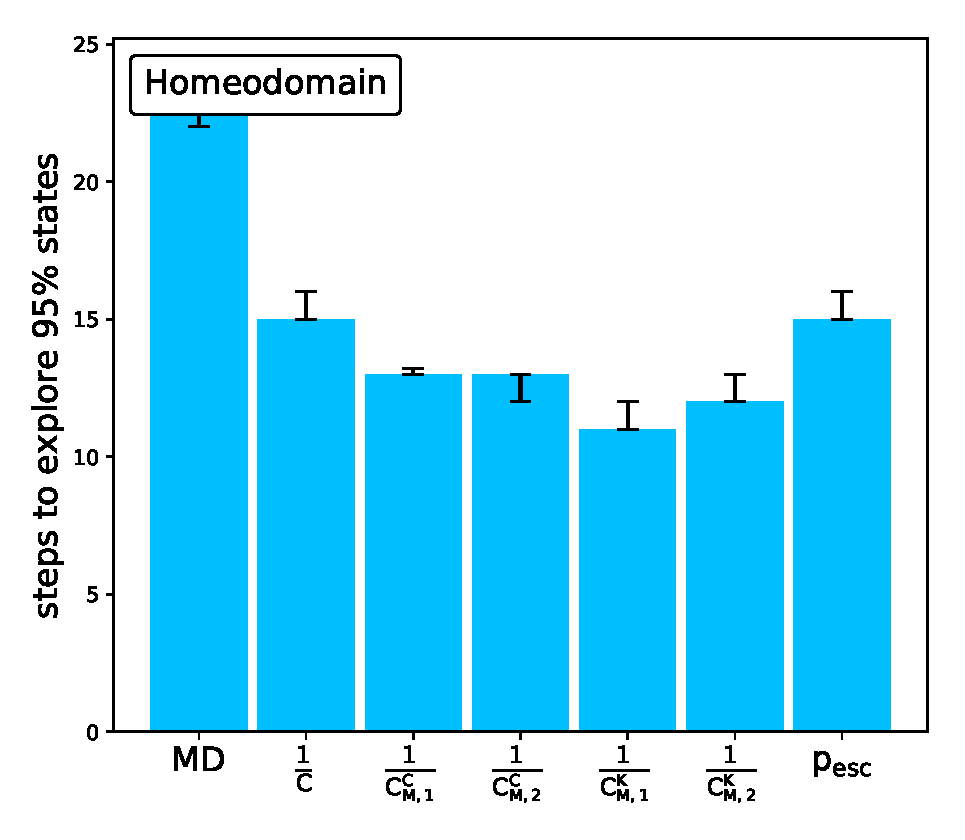
\includegraphics[width=\linewidth]{figures/UVF_7_steps10000_nparallel100_explore.eps}
  \caption{Exploration of the protein energy landscape in TICA coordinates. The
 color background shows the explored Free Energy landscape by the reference
 dataset. The black diagonal lines on top show the explored conformations by the adaptive
 sampling in this paper. The almost perfect overlap shows that the whole
 conformational landscape of \GRE{all 4 proteins was fully explored. The labels show} the location of the folded state. Individual proteins: A) Chignolin B) Villin }
\end{figure}

\begin{figure}[h!]\ContinuedFloat

   
   \begin{subfigure}[b]{0.85\linewidth}
   {\scalebarimg{figures2/plot_reana_61_extasy_vamp_bba3-cmicro-free-energy-TICA2-overlap_mod.pdf}{0.98}{C)}{0mm}{-2mm}}
   \end{subfigure}%
  
   \begin{subfigure}[b]{0.85\linewidth}
   {\scalebarimg{figures2/plot_reana_61_extasy_a3d9-free-energy-TICA2-overlap_mod.pdf}{0.98}{D)}{0mm}{-2mm}}
   \end{subfigure}%

  %%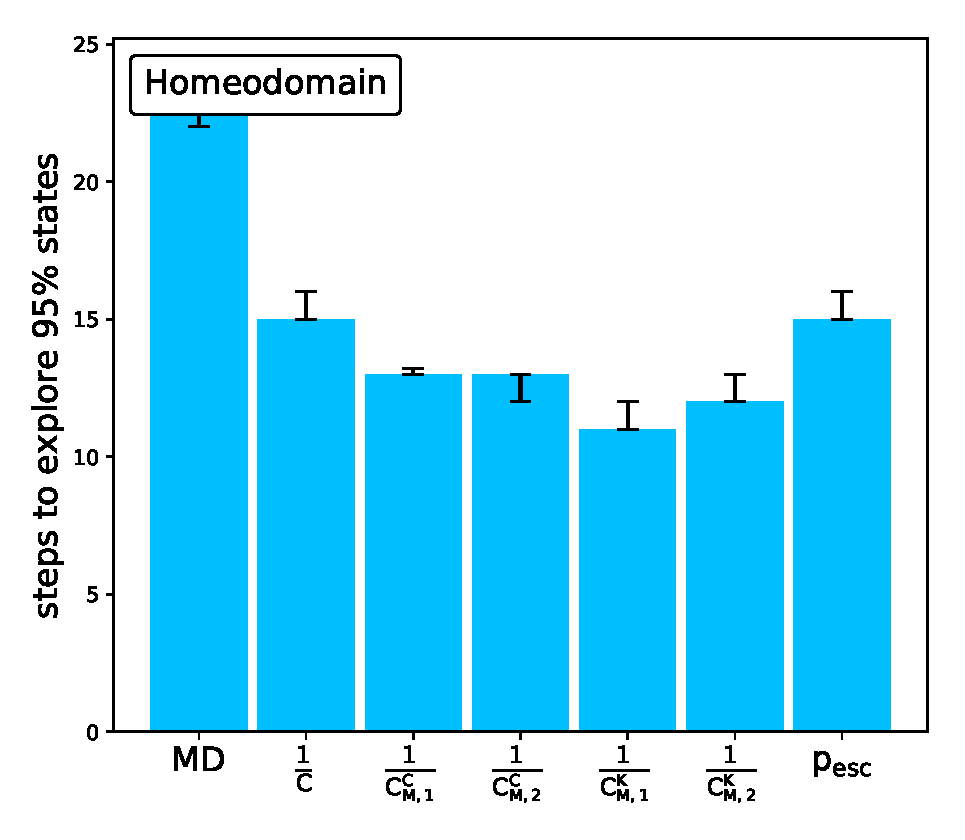
\includegraphics[width=\linewidth]{figures/UVF_7_steps10000_nparallel100_explore.eps}
  \caption{\GRE{(cont.)} Individual proteins: C) BBA \GRE{D) A3D}} 
  \label{fig:overlap}
\end{figure}

The MD simulations in this work were performed with \GRE{OpenMM 7.5} \cite{openMM}
using \GRE{CUDA 9.1 on the Summit supercomputer}. To reproduce the same setup
as in \cite{lindorff2011} we used CHARMM22* force field \cite{Charmm22star}
and the modified TIP3P water. The stepsize used was 5fs \GRE{or 2fs in case of protein A3D}, and the trajectories
were strided to \GRE{ to reduce the data volume}. Differently
from \cite{lindorff2011}, we used the Particle Mesh Ewald method for
long-range electrostatics due to OpenMM \GRE{settings}. For each protein, the start \GRE{configuration
is one frame in the reference dataset selected randomly from the 20\%
of frames with the highest Root Mean Square Deviation (RMSD) from the
protein crystal structure.} A short energy equilibration (1-2ns) was then
performed in the NPT ensemble to create initial coordinates for the workflows.
No further a priori information was given to the ExTASY framework except the
unfolded start conformations.

In each iteration, 50 OpenMM trajectories were simulated on 50 \GRE{GPUs on Summit with one GPU per trajectory. The length of each trajectory was 50ns
for Chignolin and Villin, 10ns for BBA and 40 ns for A3D. ExTASY scales up to
1000s of GPUs, so it} can be used to simulate even larger proteins or \GRE{a larger number of parallel walkers}.  Steps 2 and 4 were performed on \GRE{one GPU on Summit utilizing the same job as the MD simulations.}  After all the simulations are finished, the folding times, speed up and the accuracy of protein dynamics was determined by
comparing with the Anton MD simulations starting from the selected start
conformation. 
\GRE{In this paper, we illustrate the abilities of adaptive sampling and the ExTASY framework by comparing the results of adaptive sampling and plain MD for the 4 proteins. The expected variation of the time to fold for both adaptive sampling and plain molecular dynamics can reach 50\% \cite{Adstrategies2018}, caused by stochasticity. A significant increase of computational resources would be required to make the comparison between adaptive sampling and plain MD statistically significant.}


\begin{figure}[h!]
   \begin{subfigure}[b]{0.8\linewidth}
   {\scalebarimg{figures2/plot_chigsummary14_pop_fraction2_2_mod3.pdf}{0.95}{A)}{0mm}{-5mm}}
   \end{subfigure}%
   
   \begin{subfigure}[b]{0.8\linewidth}
   {\scalebarimg{figures2/plot_vilsummary14_pop_fraction2_2_mod3.pdf}{0.95}{B)}{0mm}{-5mm}}
   \end{subfigure}%


  \caption{The population of explored states evolving with absolute simulation time.  Around one
  order of magnitude shorter time to solution can be reached with adaptive
  sampling compared to plain MD simulations. \GRE{For Chignolin and A3D the $cmacro$ adaptive sampling strategy was used, for Villin and BBA the $cmicro$ adaptive sampling strategy was used. Both adaptive sampling strategies are described in Section~\ref{sec:restart-strategies}. The vertical lines indicate folding events.} Individual proteins: A) Chignolin B) Villin }
\end{figure}

\begin{figure}[h!]\ContinuedFloat
   \begin{subfigure}[b]{0.8\linewidth}
   {\scalebarimg{figures2/plot_bbasummary14_pop_fraction2_2_mod3.pdf}{0.95}{C)}{0mm}{-5mm}}
    \end{subfigure}%

   \begin{subfigure}[b]{0.8\linewidth}
   {\scalebarimg{figures2/plot_a3dsummary15_pop_fraction2_2_mod3.pdf}{0.95}{D)}{0mm}{-5mm}}
    \end{subfigure}%
  \caption{
  \GRE{(cont.) Proteins C) BBA D) A3D } \GRE{The plain molecular dynamics simulation of A3D has not folded despite simulating about 7 times longer than necessary for folding with adaptive sampling. Additional computational resources would allow to fold protein A3D with plain molecular dynamics too.}}
  \label{fig:Pop_explored}
\end{figure}
\section{\label{sec:results}Results and Discussion}

To analyze the efficiency of adaptive sampling, we considered several
measures. To show the completeness of the exploration, we measured the fraction
of the explored population and considered the overlap of the explored areas with the
reference dataset. This also allows us to estimate the speed up time to solution
compared to the reference method. To analyze the accuracy of the simulated
protein dynamics we compare the relative entropy of the MSM transition
matrices, and the Mean First Passage Time (MFPT) to the folded state, as
detailed below.

\subsection{\label{sec:time-fold}Comparison of Exploration}
\begin{figure}[!htb]
   
   \begin{subfigure}[b]{0.85\linewidth}
   {\scalebarimg{figures2/plot_vilsummary14_rel_ent_fold_4_mod2.pdf}{1}{}{0mm}{-3mm}}
   \end{subfigure}%
   
  \caption{
  Relative entropy between the MSM transition matrices generated during the
  ExTASY exploration and from the \GRE{plain MD comparison run}. Results \GRE{for protein Villin}. The relative entropy decreases with increasing number of adaptive
  sampling iterations. }
  \label{fig:rel_ent}
\end{figure}

The whole explored energy landscape of the protein cannot be visualized due to
the high dimensionality of the raw trajectories, but the explored landscape in
the reduced TICA coordinates is shown in
Figure~\ref{fig:overlap}. The colored background shows the explored free energy landscape of
the reference dataset and the shaded foreground shows the region of this landscape explored
by the adaptive sampling. The whole energy landscapes of the proteins\GRE{ Chignolin, Villin, BBA and A3D were} explored by ExTASY. The small differences in overlap could be
caused by the differences in the long-range electrostatics setup and stochastic \GRE{nature of the exploration}. The case of protein A3D shows that for larger protein the computational resources to fully explore the energy landscape rise significantly. \GRE{Our computational resources allowed us to fold A3D with adaptive sampling, but not with plain molecular dynamics. The plain molecular dynamics simulation didn't fold even when simulating about 7 times longer than the time to fold with adaptive sampling. To show that adaptive sampling works with different adaptive sampling strategies, we folded Chignolin and A3D with the $cmacro$ adaptive sampling strategy and  the $cmicro$ adaptive sampling strategy was used to fold Villin and BBA.}

To show how effectively the whole protein landscape is explored, we
use the fraction of the total population explored as a function of time.
Here we select all the states which are explored at a certain time and
compare with all possible states (as obtained from the reference simulations).
To represent the different importance of different states we weight the
explored states with their stationary weight. The population of each microstate
is calculated as the stationary weight of that microstate from the MSM analysis of
the reference dataset. Figure~\ref{fig:Pop_explored} reports the comparison of
the explored populations as a function of time for the reference dataset and
the ExTASY results. \GRE{For all 4 proteins, adaptive sampling explores the protein energy landscape slightly faster and folds significantly faster. The folding speed up of adaptive sampling compared to plain MD is 170\% for Chignolin, 20\% for Villin, 380\% for BBA, and more than 690\% for A3D. The larger speed up for A3D is in line with the prediction that for larger and more complex protein adaptive sampling achieves a larger speed up\cite{Adstrategies2018}. The exact speed up for the protein A3D could not be determined due to limited computational resources. The quantitative comparison between adaptive sampling and plain MD is not statistically significant due to the low sample size caused by limited computational resources.}

The x-axis in Figures~\ref{fig:Pop_explored}-\ref{fig:mfpt}
is absolute simulation time to show the improvement of time to solution with ExTASY.
Absolute simulation time is the length of one trajectory in Step 1 times the number of iterations.
When all the trajectories in Step 1 are run in parallel, the absolute simulation time
shows the time to solution independent of the used hardware. The effects of parallelization
on the time to solution for adaptive sampling were explored in \cite{Adstrategies2018},
generally \GRE{parallelization} decreases the time to solution.

\begin{figure}[!htb]
   \begin{subfigure}[b]{0.87\linewidth}
   {\scalebarimg{figures2/plot_chigsummary14_mfpt_unfold_3_mod2.pdf}{1}{A)}{0mm}{-2mm}}
   \end{subfigure}%
   
   \begin{subfigure}[b]{0.87\linewidth}
   {\scalebarimg{figures2/plot_vilsummary14_mfpt_unfold_3_mod2.pdf}{1}{B)}{0mm}{-2mm}}
   \end{subfigure}%
   
   \begin{subfigure}[b]{0.87\linewidth}
   {\scalebarimg{figures2/plot_bbasummary14_mfpt_unfold_3_mod2.pdf}{1}{C)}{0mm}{-2mm}}
    \end{subfigure}%
  \caption{
  MFPT from \GRE{folded to unfolded states evolving as
  more data is available after more adaptive sampling iterations. The red line is adaptive sampling, the blue line is plain MD with the same parallelization as adaptive sampling. The black dashed line shows the reference values for Anton simulation trajectories\cite{lindorff2011}.}   
  Individual proteins: A) Chignolin B) Villin C) BBA } 
  \label{fig:mfpt}
\end{figure}

\subsection{\label{sec:kinetics}Comparison of Protein Dynamics}


To track the convergence of protein dynamics in the adaptive sampling workflow,
one can use the relative entropy \cite{bowman2010enhanced} between the
MSM transition matrix of the reference data, $P_{ij}$, and the MSM transition matrix
of the analyzed data, $Q_{ij}$.
A relative entropy can be calculated between each microstate in the analyzed
and the reference transition probabilities from this state. By averaging the
relative entropy for each state weighted by the stationary probability over all
microstates we obtain the relative entropy between the two transition matrices.
The relative entropy
$D(P||Q)$ is then given by
\begin{equation}
D(P||Q)=\sum_{i,j}^{N}s_{i}P_{ij}\ln\frac{P_{ij}}{Q_{ij}}. 
\end{equation}
where $s_{i}$ is the equilibrium probability of state $i$. The transition
matrices $P_{ij}$ and $Q_{ij}$ have to use exactly the same dimension reduction
and same clustering.
As zero counts in the transition matrices can cause divergence of the relative
entropy, a pseudo-count of $1/N$ (where $N$ is the length of the simulation) is
added to each element of the count matrices
before normalizing the rows to get the transition matrices
\cite{bowman2010enhanced}. \GRE{ The relative entropy for a certain simulation time is
obtained from all the trajectories up to the specified simulation time. By definition, the relative entropy of the full reference
trajectory is zero.  Figure~\ref{fig:rel_ent} shows how the relative
entropy decreases with increasing simulation time for both the adaptive sampling and plain MD simulations. The adaptive sampling strategy decreases the relative entropy faster at the beginning, later in the simulation plain MD decreases the relative entropy faster. While the sample size is small, this confirms that the chosen investigated sampling strategy is effective at exploring the protein landscape, but not optimized in the later steps of converging protein kinetics \cite{Adstrategies2018}. Different adaptive sampling strategies which are optimized for converging the kinetics could improve the behavior of adaptive sampling towards the end of the simulation.}

\GRE{An additional measure to compare the convergence of the kinetic behavior of the proteins is Mean First Passage Time (MFPT). MFPT measures the mean time to reach for the first time another state from one state. Here the two states are the folded and unfolded states, both defined as an ensemble of MSM states based on the TICA coordinates. The folded and unfolded MSM states for the proteins were
defined by their TICA positions. Figure~\ref{fig:mfpt} shows how the MFPT from the
folded to the unfolded state converges as a function of simulation time, for both the adaptive sampling and the plain MD simulations. The reference MFPT obtained from Anton trajectories shows that the results of both plain MD and adaptive sampling can be about one order magnitude off the reference value. Adaptive sampling shows larger errors in the case of Chignolin and Villin, but a smaller error in the case of BBA compared to plain MD. The small sample size prevents us to conclude if plain MD or adaptive sampling converges faster. Additionally, the used adaptive sampling strategies are not optimized or validated for convergence of kinetics. The slow convergence of MFPT for Chignolin and Villin shows that accurate kinetic values require a long sampling and that kinetic values from both plain MD and adaptive sampling have relatively large uncertainties. The sizes of the MFPT errors are similar to what was obtained with the HTMD framework \cite{doerr2016htmd}. For protein A3D the convergence of MFPT could not be compared since the plain MD simulation did not fold. Additional investigation in the theory of convergence of kinetic values for protein sampling methods would allow understanding these results better.}  


\section{\label{sec:conclusion}Conclusion}

We have shown that the ExTASY framework \cite{Extasy2016} can effectively
perform adaptive sampling, as exemplified \GRE{by adaptively sampling 4 proteins using deep learning. The free energy landscape of the 4 proteins was fully sampled. In comparison to a plain molecular dynamics simulation with the same parallelization a small but not statistically significant speed up in the range of 20\% to 690\% could be observed. These speed ups are in line with predictions \cite{Adstrategies2018} which rise with the size of the proteins. The MFPT times converged for both adaptive sampling and plain MD to values similar to the reference values. For protein BBA the adaptive sampling converges the MFPT significantly faster than plain MD, but proteins Chignolin and Villin show as slower convergence. The expected large stochastic fluctuation expected in both plain MD and adaptive sampling prevents a statistically significant comparison of MFPT times between plain MD and adaptive sampling. The sample size in this paper was limited by computational resources. Additional adaptive sampling strategies optimized in recovering the kinetics would improve the results of adaptive sampling for MFPT convergence. The relative entropy between the transition matrix of the MSM computed during the adaptive
sampling and the MSM of the plain MD decreases steadily with the
simulation time, the adaptive sampling converges here faster than plain MD at the beginning of the simulation. The differences in speed of convergence are caused by the choice of adaptive sampling strategy, which are validated for the exploration of protein energy landscapes, but not optimized to reach accurate protein kinetics. Due to the stochasticity, the comparison of the speed up between adaptive sampling and plain MD is not statistically significant. For statistically significant results a significant increase in computational resources would be required.}
\GRE{The modularity of the ExTASY framework reduces the time spent by domain experts in executing
adaptive sampling in a scalable fashion on diverse platforms. Scalability of over 1000 GPUs and 1000 simultaneous protein replicas was demonstrated on Summit. This scalability doesn't come at the cost of inflexibility, due to the design and implementation of the ExTASY framework \cite{Extasy2016}, ExTASY can be
easily modified for different proteins or MD
simulation software. ExTASY can also be easily extended to different adaptive
sampling strategies and platforms. The ExTASY framework is available open-source at} \href{https://github.com/ClementiGroup/ExTASY}{https://github.com/ClementiGroup/ExTASY}. \GRE{The flexibility of ExTASY allowed this framework to be the first open-source adaptive sampling platform which supports deep learning or asynchronous execution.}
